\subsection{PULL (32)}

The PULL message requests IPv4 addresses of other nodes in order to expand its
list of neighbors. This message can be sent to an existing neighbor or a DNL
node. The number of addresses returned can be smaller than the number of
addresses requested. The list of addresses from the reply can be missing if the
status code indicates an error.

\begin{figure}[H]
    \centering
    \scalebox{.33}{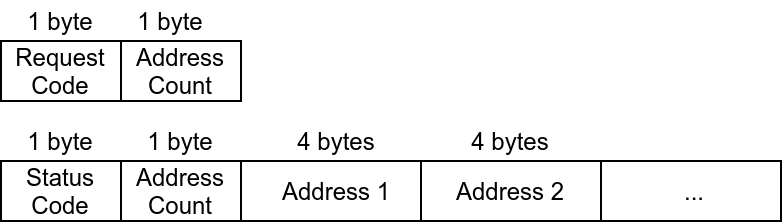
\includegraphics{figures/pull}}
\end{figure}

\subsection{PUSH (33)}

PUSH can be sent by a node to make itself known to its new neighbors of which
addresses were retrieved using the PULL message. The nodes which are receiving
this message will add the address of the message source to its list of
neighbors.

\subsection{BYE (34)}

BYE should be sent by a node to notify its neighbors and one of the DNL nodes
that it will leave the network so they can remove the node from the neighbor
list and perform proper cleanup. There is no reply for this message.

\subsection{DEAD (35)}

Used to notify a node's neighbors and DNL nodes that some other nodes were 
found to be dead (not responding). These dead nodes did not send the BYE 
message before leaving (this may be due to a software crash or power failure). 
The nodes which are receiving this message should check if the specified nodes
are indeed dead by pinging before removing them from the neighbor list.

\begin{figure}[H]
    \centering
    \scalebox{.33}{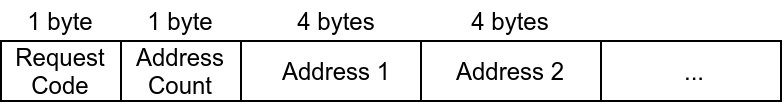
\includegraphics{figures/dead}}
\end{figure}

\subsection{PING (36)}

PING is used in conjunction with the DEAD message. Pings a node to confirm that
it indeed left the network without sending the BYE message.

\subsection{DNLSYNC (37)}

This is a special message sent between DNL nodes to synchronize the distributed 
data structure. Updates are accumulated and periodically sent in bulk using a 
single message. The message data itself contains a list of entries, each 
representing an update. An entry contains the type of the action (0 for 
\textit{Add Address} and 1 for \textit{Remove Address}) , the address to be 
added or removed and the time point at which the action was originally 
performed. The timestamp is crucial for resolving potential conflicting updates 
- for example a DNL node informs the others that a peer has joined the network 
while another informs that it left instead.

\begin{figure}[H]
    \centering
    \scalebox{.33}{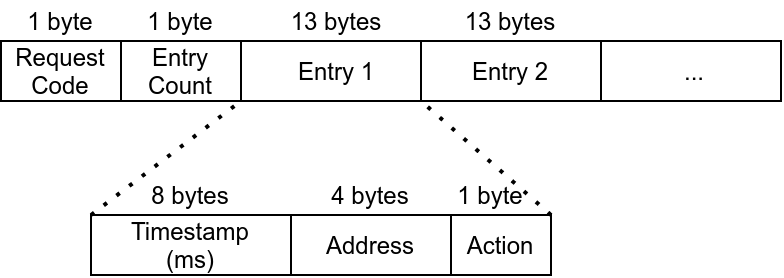
\includegraphics{figures/dnlsync}}
\end{figure}
